\subsection{Nebulas Virtual Machine (NVM)}
\label{sec:nvm}

We will introduce LLVM \cite{llvm} as the main component of NVM and
LLVM bytecode as the NVM bytecode. The NVM bytecode is dynamically
compiled and optimized through LLVM JIT and is executed in the NVM sandbox environment. With this architecture design, the performance and security of the core code and the smart contract of Nebulas can be continuously improved with the introduction of LLVM. 

%我们将引入LLVM~\cite{llvm}做为NVM的核心组件,并使用LLVM Byte Code做为NVM字节码。NVM字节码通过LLVM JIT完成动态编译和优化,运行在NVM沙盒环境中。在这种架构设计下,星云链的核心代码、智能合约能直接享受到LLVM带来的性能和安全性的不断提升。

LLVM is a collection of highly modularized compiler toolchains and
technologies, which was used as a code compilation framework in Google, Apple
and many other companies. LLVM provides neutral intermediate representations
(LLVM IR) and the corresponding compilation infrastructure, and offers a brand
new set of compilation strategies regard to these infrastructure, including
optimization of LLVM IR, code generation from the LLVM IR to the LLVM bytecode
and direct execution of the LLVM bytecode in different hardware platforms via
the LLVM JIT, shown in \reffig{fig:llvm}. \\

%LLVM早期是Low Level Virtual Machine的缩写,是一系列高度模块化的编译器和工具链技术的集合,包括Google、Apple在内的公司都使用它做为代码编译框架。LLVM提供了一套中立的中间表示(LLVM IR)和相应的编译基础设施,并围绕这些设施提供了一套全新的编译策略,包括对LLVM IR的优化、LLVM IR到不同硬件平台的代码生成、LLVM IR到LLVM Byte Code的代码生成以及LLVM Byte Code在不同硬件平台上通过LLVM JIT直接执行。如图\ref{fig:llvm}所示

\begin{figure}[h]
\centering
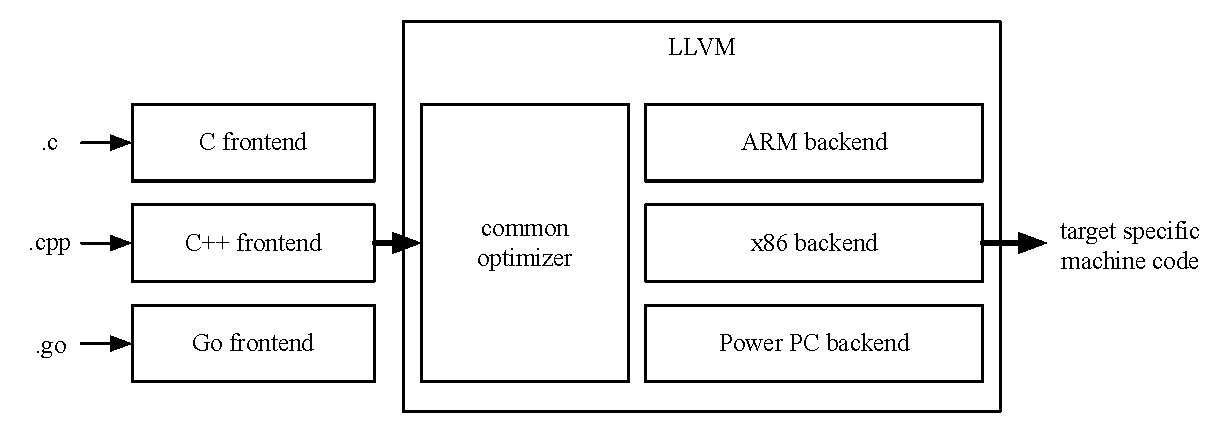
\includegraphics[width=10cm]{./figs/llvm}
\caption{LLVM}
\label{fig:llvm}
\end{figure}

We construct the NVM based on LLVM, shown in \reffig{fig:nvm}. First
of all, we provide the underlying API libraries for blockchains. After that, we
construct compiler frontend for different languages, such as Solidity,
JavaScript, C/C ++, Go, etc. Then, we use the toolchain provided by LLVM to
generate the LLVM bytecode. Finally, the LLVM bytecode is executed in a safe
sandbox environment provided by NVM through JIT engine of LLVM.

% 我们依托LLVM构建NVM,如图\ref{fig:nvm}所示。首先,我们提供区块链底层API库;然后,我们为不同语言(如Solidity,JavaScript,C/C++,Go等)构建生成LLVM IR的编译器前端;最后,利用LLVM提供的工具链,生成LLVM Byte Code。最终,LLVM Byte Code通过LLVM的JIT引擎运行在NVM提供的安全的沙箱环境中。

\begin{figure}[h]
\centering
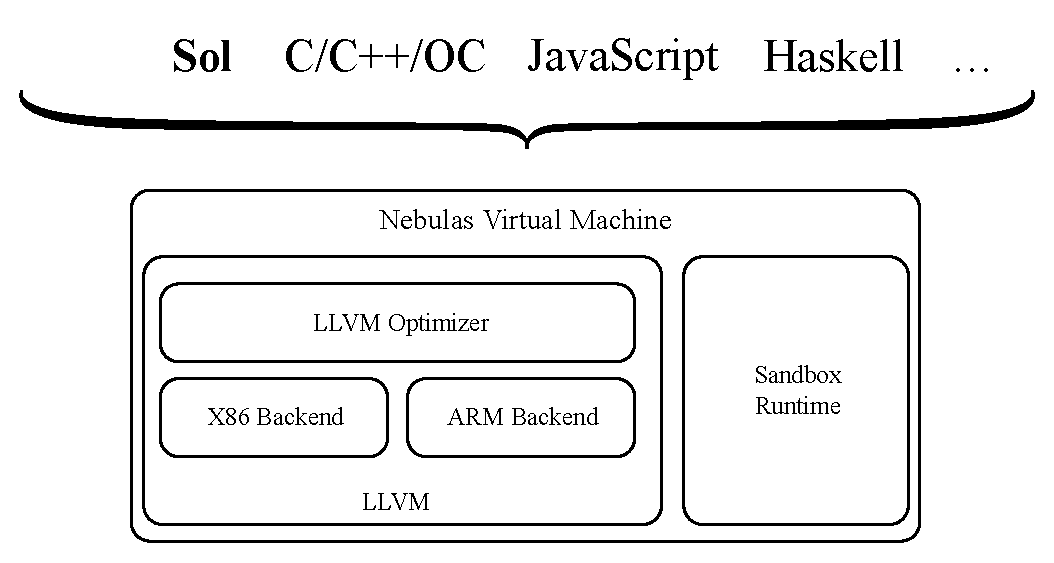
\includegraphics[width=10cm]{./figs/nvm}
\caption{Nebulas Virtual Machine}
\label{fig:nvm}
\end{figure}

NVM is an important cornerstone of the Nebulas Force. When any new protocol
code or smart contract is released, the LLVM bytecode is generated after the
new code is complied by the LLVM compiler module in NVM and is released to the
chain. After confirmed on chain, the new code will be complied and
optimized by LLVM JIT, and then into the sandbox to replace the old code and
be executed, shown in \reffig{fig:nvm-process}.

%NVM是星云原力的重要基石。新的协议代码或智能合约发布时,NVM中LLVM编译器模块完成新代码的编译得到LLVM字节码,然后发布到链上;链上确认后,新代码将由LLVM JIT完成编译和优化,然后进入沙箱取代旧代码并被执行,过程如图\ref{fig:nvm-process}所示。

\begin{figure}[h]
\centering
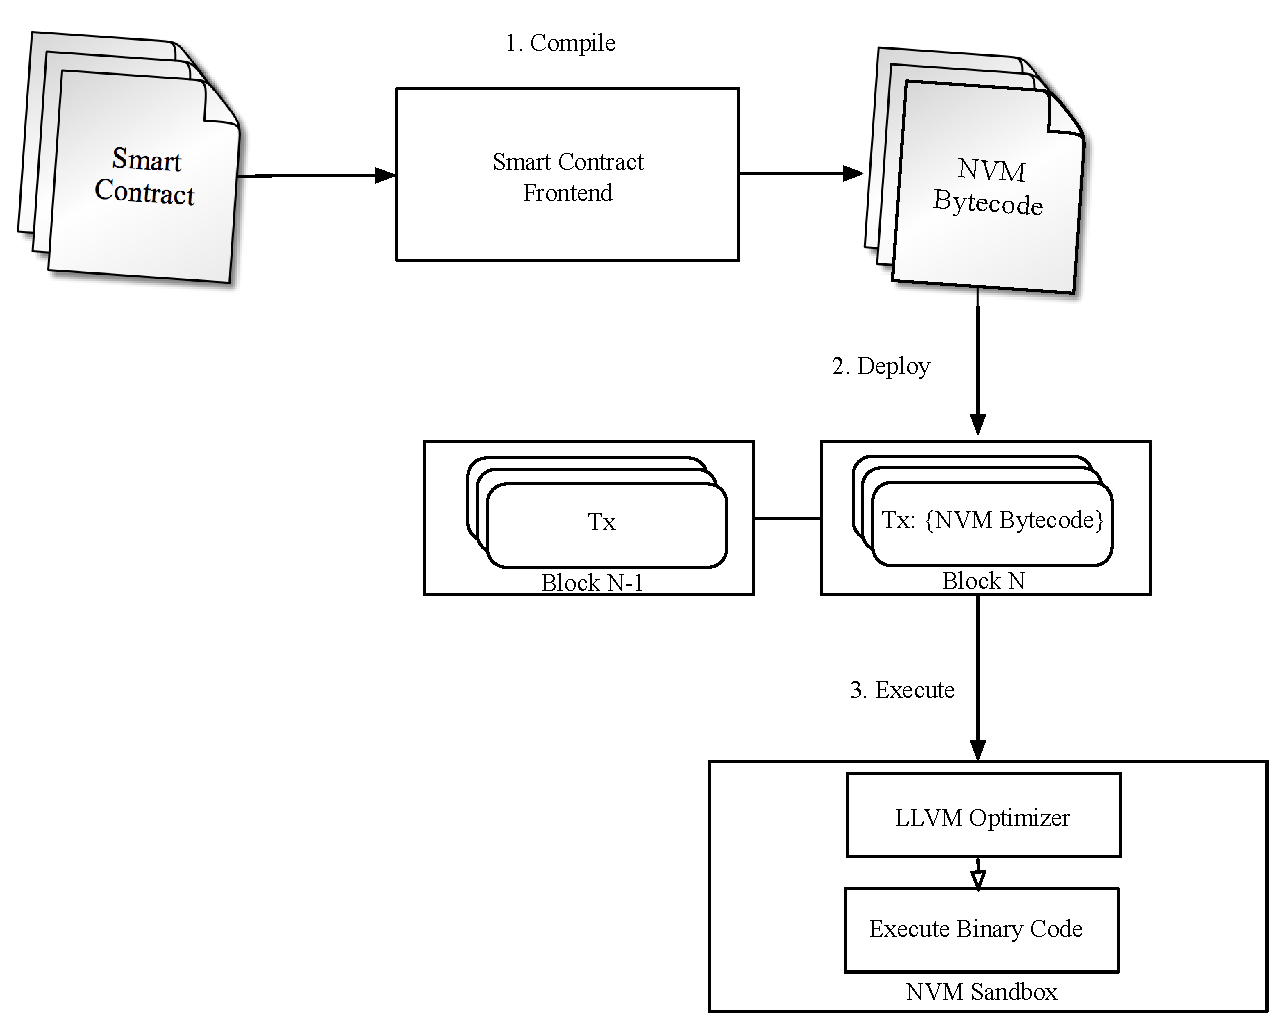
\includegraphics[width=10cm]{./figs/nvm-process}
\caption{The operation mechanism of the Nebulas Virtual Machine}
\label{fig:nvm-process}
\end{figure}

With LLVM (see \reffig{fig:llvm}), NVM also supports developers to develop
smart contracts and applications with their familiar programming languages,
such as Solidity, more flexible JavaScript, and even pure functions type of
language Haskell. In addition to these popular languages, NVM can also provide
customized high-level languages for different areas and scenarios, such as DSL
(domain-specific language) for financial systems. These high-level languages
are easier to be formally verified, further improving code robustness and
security, and more conducive to the developers developing richer Smart contract
and application.

%借助于LLVM(见\ref{fig:llvm}),NVM还支持开发者用其熟悉的编程语言开发智能合约和应用,比如以太坊智能合约所使用的Solidity,更加灵活的JavaScript,甚至是纯函数式语言Haskell。除了这些通用语言外,NVM还可以为不同领域和场景提供定制的高级语言,比如面向金融行业的DSL(领域专有语言)。这类高级语言面向行业、场景高度定制,使得它们更容易被形式化验证,能进一步提高代码健壮性和安全性,更有利于星云链开发者开发出更丰富的智能合约及应用。
